\section{Overview}

\todo[inline]{Answer this question: how many references do you want here? How
many are you going to delay until the lit review?}

\todo[inline]{Short paragraph, non-rigorous definition of plasmas. Be sure to
  clarify distinction from electrical discharge, or if you consider them the
same.}

Historically, the study of atmospheric-pressure plasmas (\acs{app}'s) is
indistinguishable from the study of plasmas as a whole. However, the detail of
the measurements and calculations associated with \acs{app}'s has been limited
by their complexity. From a computational perspective, the high pressure and
number of potential reactions present a difficult challenge. Likewise, the high
pressure can significantly complicate the data analysis for a number of plasma
diagnostics. Aside from the high pressures, the large electric fields, short
time scales, and general randomness of \acs{app}'s make even the most basic
observations a feat.

\todo[inline]{Ambiguous start to paragraph, specify and cite problems, then
identify how they have been overcome.}

In the last several decades, some of this has begun to change. High-powered
computing has allowed simulations with remarkable detail. Similarly, advances in
technology has enabled plasma diagnostics in regimes that were experimentally
inaccessible. As a result, the body of knowledge regarding \acs{app}'s has
greatly increased. Sometimes, the motivation for this work is scientific
curiosity. More often, the study of \acs{app}'s has been driven by a broad range
of applications.

Among the first plasma applications were provided by \acs{app}'s: ozone
generation and lighting. Aside from these items, plasma welding, polymer
treatment, combustion, and plasma televisions have become widely accepted.
Meanwhile, a large number of new applications may soon be added to this list,
including: treatment of tissue wounds, altering airflow over airfoils, and
destruction of industrial pollutants.

Unsurprisingly, each case demands a different kind of plasma. The original arc
discharges were created between two graphite rods connected to immense battery
banks. In contrast, a modern research reactor studying plasma-assisted
combustion might use a fast-switching semiconductor circuit. Over the years,
several types of \acs{app}s have been developed for a variety of situations:
dielectric-barrier, corona, thermal arc, RF, microwave, pulsed, and more.

Within this group\footnote{The interested reader is referred to Starikovskaia's
review \cite{Starikovskaia2006} which provides a general overview of \acs{app}'s
in the context of plasma-assisted combustion}, the repetitively-pulsed
nanosecond discharge (\acs{rpnd}) has created considerable interest. Generally
speaking, a \acs{rpnd} is a plasma generated by a repetitive electrical pulse
applied between two electrodes. The pulse voltage is often in excess of one
kilovolt, lasts anywhere from $<1-100$ ns, and is repeated over a thousand
times each second. The result is a wave of ionization (and light) which crosses
from the powered electrode to the grounded one.

A \acs{rpnd} can fill volumes of several liters with a relatively uniform
plasma. Though they can cause significant excitation of the background gas, they
generally produce very little heating (in some cases below a detection limit of
$\Delta \pm 15$ K). In addition, the excitation can be changed with adjustments
to the magnitude or duration of the electrical pulse. Each of these
characteristics are highly desirable in one or more of potential applications
for \acs{app}'s.

Given all of these promising properties, \acs{rpnd}'s have been the subject of
substantial study by several research groups. However, much of this work has
focused on the physics of \acs{rpnd}'s in air. Unfortunately, air's large number
of constituent elements can lead to notable complexity. In turn, this can
obscure some of the more fundamental questions relation to \acs{rpnd}'s: how do
they form, how is the energy distributed between excited particles, and what
kind of spatial variation can be expected?

This paper details a study of each of these questions in a helium \acs{rpnd}.
Specifically, the densities of one particular excited atom are measured for a
variety of pressures and locations. This is complemented by measurements of the
light emissions for the same set of parameters. A simple model of a \acs{rpnd}
is used to predict several characteristics of the plasma based on the excited
state densities: electron density, electric field, and light emission. The
measured light emissions are interpreted to show how the energy is distributed
in the gas, and how it changes over time. Finally, they are compared with the
estimated light emissions to check the validity of several common assumptions.

\todo[inline]{Paragraph on reason for choosing helium, specify choice of
measurements and topic of dissertation}

The remainder of this chapter is comprised of a review of the associated
literature, as well as a discussion of basic discharge theory. Chapter
\ref{chp:exp} covers the experimental setup as well as some general observations
of the \acs{rpnd}. Next, the measurement of the excited state densities is
presented, followed by the chapter on the light emission measurements. Chapter
\ref{chp:model} explores the global model used to interpret the excited state
densities, as well as some supporting particle-in-cell simulations. Finally, the
paper concludes with a discussion of how the models and measurements impact the
present understanding of \acs{rpnd}'s.

\section{Literature Review}

Though \acs{rpnd}'s are very much a product of twentieth century research, they
are fundamentally similar to a number of other pulsed discharges such as
electrical sparks and lightning. Though Loeb united these disparate fields under
the title of ``ionizing waves of potential gradient'' in 1964 \cite{Loeb1965}
(we use the more familiar term, fast ionization waves), the underlying subjects
had been under study since the Greeks who generated sparks by rubbing together
amber and fur.

Despite these early observations, it was Leibniz in 1671 who first came to the
conclusion that sparks were an electrical phenomena \cite{Kryzhanovsky1989}.
Subsequently, Franklin's famous kite experiment led him to a similar conclusion
on the nature of lightning. Franklin was also involved in explaining the
principles of Leyden jars, develop by Musschenbroek. The Leyden jar was the
first reliable way to store electrical energy and proved a boon to later
research.

In 1835, Wheatstone made the first attempt to measure the speed of electricity
through a gas \cite{Wheatstone1835}. In his work, Wheatstone used a Leyden jar
connected to two metal spheres, separated by a small gap. Once the charge in the
jar reached a critical level, a spark would form in the gap. Figure
\ref{fig:wheatstone} shows the experimental sketch provided by Wheatstone.
\begin{figure}
  \centering
  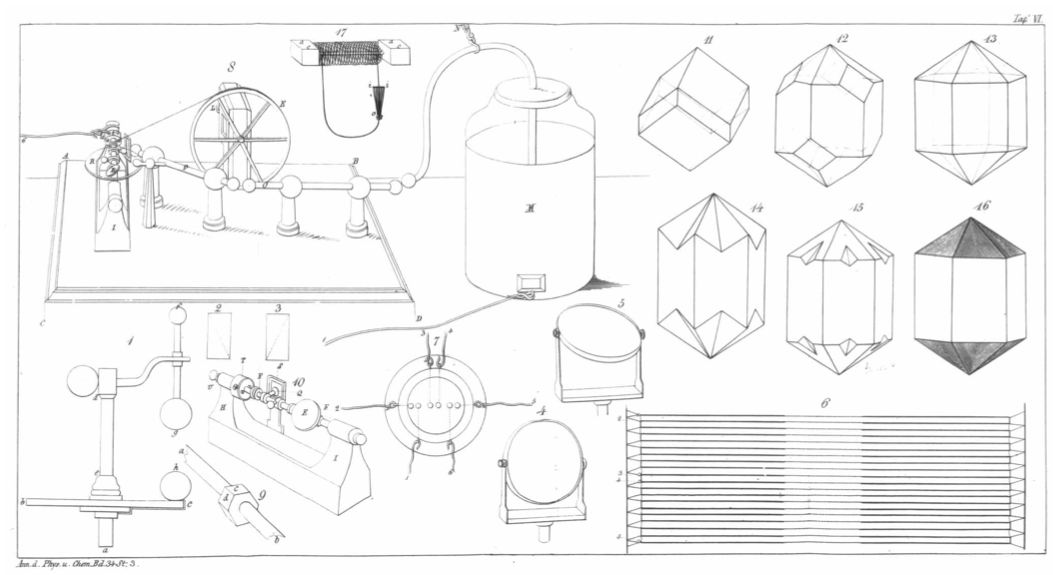
\includegraphics[width=4in]{chapters/introduction/figures/wheatstone.png}
  \caption{The experimental sketches of Wheatstone showing a traditional
  spark gap connected to a Leyden jar and electrostatic
generator.}\label{fig:wheatstone}
\end{figure}
Though the measurement is notable for its early date, it was later revisted with
much more accuracy by Thomson \cite{Thomson1893}. Perhaps the most important
outcome of Wheatstone's study was the observation by Zahn \cite{Zahn1879} that
the speed of the light was \emph{not} accompanied by a similar motion of the
emitting particles.

Thomson's work concerned both the speed and direction of light in a pulsed
discharge. Unlike Wheatstone's study, Thomson used an elongated tube, 15 m in
length, and 5 mm in diameter, upon which he drew a vacuum. The original sketch
of Thomson's discharge apparatus can be seen in figure \ref{fig:thomson}.
\begin{figure}
  \centering
  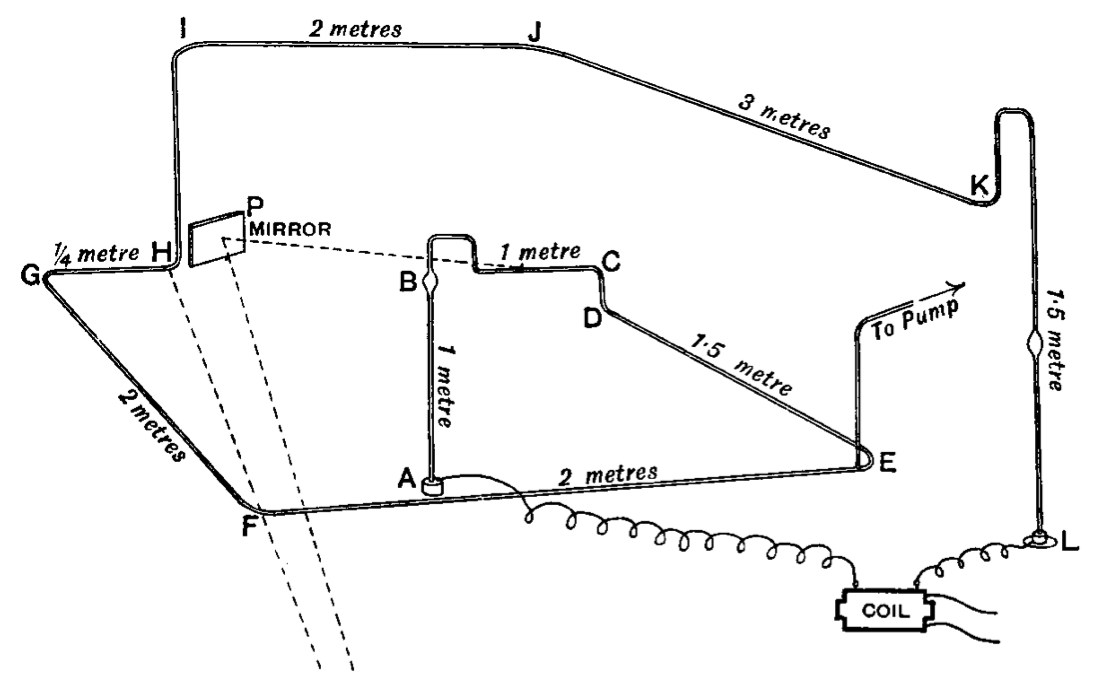
\includegraphics[width=4in]{chapters/introduction/figures/thomson.png}
  \caption{A sketch of J.J. Thomson's early experiments on fast ionization
  waves in long vacuum tubes.}\label{fig:thomson}
\end{figure}
Through a clever arrangement of mirrors, Thomson determined that the electricity
had a speed approaching $1\times10^{10}$ cm/s, and travelled from the anode to
the cathode.

It was later, in 1930, that Beams would determine that the wave always initiated
at the high voltage electrode, regardless of polarity \cite{Beams1930}. In
addition, Beams measured the current at the low potential electrode. He detected
a current pulse which did not appear until after the light had completely
crossed the gap. He came to the conclusion that the luminous front was likely
the result of a moving region of ionization.

Around the same time, there was a distinct set of researchers ho were studying
similar phenomena in lightning. In most cases, these studies concentrated on
time-resolved photography, pioneered by Boys\footnote{In the same article, Boys
anticipated a number of other atmospheric physics studies by proposing that
rockets be fired at thunderclouds. Unfortunately, he lived in a village of
thatched houses and could not conduct the experiment for fear of
fire.}\cite{Boys1926}, and refined by Schonland \cite{Schonland1935}. This
technique was later adopted by Allibone and Meek \cite{Allibone1938} to observe
the evolution of a laboratory-generated spark.

\todo[inline]{Perhaps address the theory of rpnds separately?}

By 1935, fast ionization waves had been under study for nearly 50 years.
However, there was still no adequate explanation for the speed of the discharge.
Similarly, Beams' observation that the wave always travelled from the high
voltage to the low voltage electrode (regardless of polarity) was inconsistent
with the Townsend model used to explain most plasmas. Based on observations made
with fast pulses, Flegler and Raether developed a new theory of breakdown for
sparks in air \cite{Flegler1936} which was capable of, at least partly,
explaining the fast ionization wave phenomena. Independently, Loeb and Meek
developed a similar theory in 1940 \cite{Loeb1940}.

The work of Fleger and Raether as well as Loeb and Meek, was intended to explain
the breakdown processes for an undetermined range of overvoltages (in excess of
the breakdown voltage). However, as early as 1951, Fisher and Bederson
\cite{Fisher1951}, demonstrated that the Townsend mechanism was still plausible
at low overvoltages.

In contrast, 1961 saw Fowler \cite{Fowler1961} seeking a hydrodynamic
explanation for the waves. Contrary to the stochastic and particle-based
description of the streamer breakdown, Fowler considered the luminous fronts to
be nonlinear electron acoustic waves. Though the explanation provided a fair
agreement with his observations, there were several issues with the analysis,
namely a simplified consideration of the geometry and associated field
strengths.

By 1965, Loeb himself, admits that photoionization was not insufficient on its
own to produce the observed phenomena. In his review for Nature, Loeb
identified several phenomena that exhibited similar characteristics. The
return stroke in lighting, high overvoltage breakdown in rarefied gases, and
sparks in atmosphere. Loeb was able to provide a qualitative description of the
physics involved, but ultimately deferred on any quanitative description.

The insufficiency of photionization was later reinforced by the observation of
Mesyats \cite{Mesyats1972} that the speed of the discharge processes was often
faster than the lifetimes of excited states. Again, this precluded
photoionization from providing a significant amount of preionization for the
propagation of an rpnd. Mesyats instead suggested that the large fields
generated an electron avalanche that grew much more rapidly than the typical
Townsend discharge. This was followed by an avalanche chain which further
propagated the plasma.

Later, Kunhardt \cite{Kunhardt1980} extended on Mesyats' analysis and provided a
more theoretical underpinning for it. Taking his inspiration from the group
theory used in neutron diffusion, Kunhardt explored the development of a fiw
from the perspective of ``trapped'' and ``runaway'' electrons. Previous work by
Babich and Stankevich \cite{Babich1973} inspired this by suggesting the
existence of continually-accelerated electrons at high overvoltages.

As an aside, the topic of electron beams in rare gases became of substantial
interest to researchers in the mid 1970s. Because rare gases lacked low-lying
excited states which might detrimentally absorb energy, they were favor for
laser where a population inversion could be achieved with ease. As a result, a
great deal of work went into detailing the propagation of an electron beam in
rare gases which is physically similar to the development of a fast ionization
wave. However the primary difference between

It was around this time that the topic of fiw became of substantial interest to
Russian research groups. Though much of the early work is shrouded in the mists
of language differences, it is believed that Vasilyak \cite{Vasilyak1994}
provides a fair review of the material. 

\todo[inline]{Remember to include the laser dudes! Xenon lamps!}

<<<<<<< HEAD
Come 1998, the fiw was the subject of renewed interest by a group of
researchers at the Moscow Institute of Physics and Technology
\cite{Anikin1998}. They employed several different diagnostic techniques
(photomultiplier tubes and capacitive probes) in an exceptionally
detailed study of fiws in both air and nitrogen, using a shock tube and
a bell jar. A summary of these investigations can be found in
\cite{Starikovskaia2001}. The work showed exceptionally reproducibility
of the discharge parameters at relatively low repetition rates, on the
order of tens of Hz, and evidence of runaway electrons in the
electronically excited molecular states. This work also included some of
the first approximations of the electron energy distribution function
(\acs{eedf}). This was found by comparing several paremeterized
distribution functions with the resulting excited state populations.
\todo[inline]{This is pretty damned similar to what you originally
discussed}
=======
Come 1998, the fiw was the subject of renewed interest by a group of researchers
at the Moscow Institute of Physics and Technology \cite{Anikin1998}. They
employed several different diagnostic techniques (photomultiplier tubes and
capacitive probes) in an exceptionally detailed study of fiws in both air and
nitrogen, using a shock tube and a bell jar. A summary of these investigations
can be found in \cite{Starikovskaia2001}. The work showed exceptionally
reproducibility of the discharge parameters at relatively low repetition rates,
on the order of tens of Hz, and evidence of runaway electrons in the
electronically excited molecular states. This work also included some of the
first approximations of the electron energy distribution function (\acs{eedf}).
This was found by comparing several paremeterized distribution functions with
the resulting excited state populations. \todo[inline]{This is pretty damned
similar to what you originally discussed}
>>>>>>> 0f9e83efaea6255e71c74db421bb4a3c13801ba9

This was time the population kinetics of an fiw was really examined. In this
case, it emphasized the short-lived states of nitrogen. Specifically,
\cite{Pancheshnyi1998} initially used the fiw to examine the population
of electronic states of nitrogen. Later analysis \cite{Pancheshnyi1999}
concluded that the, for a negative fiw in nitrogen, the vast majority of
the electrons were generated in the aftermath of the wave and that the
ionization did not track the luminous front. Additionally, measurements
of the conductivity suggested that the local approximation becomes
invalid in the wave front and the electron energy distribution function
resembles a beam.

The development of fid semiconductor technology in the late 1990's and
their commercialization in the early 2000's allowed the use of rpnds.
Fundamentally, these discharges were the same as the fiws that had been
studied for decades earlier. However, the much greater repetition rates
(on the order of tens of kHz), meant that the discharges could be used
in a number of previously impossible applications. Attention quickly
turned toward plasma-assisted combustion \cite{Starikoskaia2006}, mhd
energy bypass \cite{Macheret2002}, and later, plasma actuators
\cite{Adamovich2009}. Additionaly studies, related to the development of
high-pressure xenon lamps, led to several more quantitative models of
the fiw development \cite{Nikandrov2008, Tsendin2009}. These works also
contributed to a semi-analytical energy coupling model as well
\cite{Adamovich2009}.

Research efforts continued to use many of the same diagnostics as
before. The current and voltage at the powered electrode were recorded
(with varying levels of diligence), electric fields were measured with
capacitive probes, and photomoultiplier tubes were used to measure the
progress of the luminous front. The 2000's did add a few new tools to
the diagnostic arsenal. Perhaps the most common addition is the use of
ICCD's in order to record transition and broadband light. This approach
has been used to verify the reproducibility of the discharge
\cite{Adamovich2009}. Though the gate times are still too short to
capture the development of the wave, excitation profiles like those
initially demonstrated by Vasilyak\cite{Vasilyak1994} are commonly
recorded. Another, more exotic addition, has been the use of CARS. This
nonlinear technique has proven to be excellent at reproducing the
spatial temperature profiles of pulsed nanosecond discharges. This has
become particularly interesting for groups interested in applications to
fast gas heating \cite{Zuzeek2010}. Others have used CARS to explore the
electric field development of rpnds \cite{Ito2011, Mueller2010}.
Finally, another research group has used LCIF to detect the radial and
axial profiles of the metastable and electron densities in a helium
discharge. The CARS and LCIF approaches are both notable for being
active diagnostics of direct properties. This allows unprecedented time
resolution and detail.



\section{Basic Theory}

\subsection{Plasmas}

A volume containing some number of charged particles can be considered a
plasma if it meets three conditions. The first requires that the motion
of charged particles is primarily determined by the electric and
magnetic fields of the volume rather than through collisions with
neutral particles. This is classically expressed by the inequality
\begin{equation}
  \sqrt{n_\mathrm{e} e^2 / (\epsilon_0 m_\mathrm{e})} < \nu,
\end{equation}
where $n_\mathrm{e}$ is the electron density, $e$ is the fundamental
charge, $\epsilon_0$ is the permittivity of free space, $m_\mathrm{e}$
is the mass of an electron, and $\nu$ is the electron-neutral collision
frequency. The left-hand side term is called the electron plasma
frequency, it the characteristic frequency at which a plasma oscillates
in response to a perturbation.

\todo[inline]{requirements for a plasma}
\todo[inline]{Be clear about relation to Lieberman's writing!}

For a sufficiently large number of particles, the behavior of the each
species of the plasma can be described by a continuous probability
distribution function. This function, $f_\alpha(\vec{r}, \vec{v}, t)$,
describes the probability of finding a particle of species $\alpha$, at
position $\vec{r}$, The distribution function for a particle can be
determined by the Vlasov-Fokker-Planck \acs{vfp} equation,
\begin{equation}\label{eq:vfp}
  \frac{\partial f_\alpha}{\partial t} + \vec{v_\alpha}\cdot\nabla f_\alpha +
  q_\alpha \left(\vec{E} + \vec{v_\alpha}\times\vec{B}\right)
  \cdot \nabla_\mathrm{v} f_\alpha = \left( \frac{\partial f_\alpha}
  {\partial t}\right)_\mathrm{coll}.
\end{equation}
Here, $\vec{E}$ is the electric field, $\vec{B}$ is the magnetic field,
and $\partial f_\alpha/(\partial t)_\mathrm{coll}$ is a term
representing all collisions. The \acs{vfp} equation is coupled to
Maxwell's equations in order to obtain a self-consistent description of
the particle distribution and the resulting fields. In essence, this is
the Boltzmann equation from statistical mechanics, however it now
includes several changes. Vlasov replaced the original force term with
the Lorentz equation, and Fokker and Planck introduced the collision
operator on the right-hand side. This is coupled with Maxwell's
equations for a solution of the electric and magnetic fields in the
plasma.

In the absence of external fields and with only elastic collisions, the
equation admits the famous Maxwell-Boltzmann equilibrium distribution,
\todo[inline]{n for degrees of freedom? Change to something
unambiguous?}
\begin{equation}\label{eq:mb}
  f_\alpha(v) = n\left(\frac{m_\alpha}{2\pi k_\mathrm{B}T}\right)^{3/2}
    \exp\left(-\frac{m_\alpha v_\alpha^2}{2k_\mathrm{B}T}\right),
\end{equation}
where $n$ is the number of degrees of freedom, $k_\mathrm{B}$ is
Boltzmann's constant, and $T$ is the temperature. A species of particles
which possesses a Boltzmann distribution is said to be in equilibrium.
Likewise, two species with the same distribution are in equilibrium.

\todo[inline]{Should the Boltzmann-Maxwell equilibrium be pushed back to
discussion of rate equations and averaging?}

Aside from this, the \acs{vfp} equation is notoriously difficult to
solve. As a result, most plasma models use various moments of equation
\ref{eq:vfp} where the velocity dependence has been integrated out.
These moments are the basis for the two-fluid equations, the MHD
formulation, and global models. We will show the first three moments
following the notation of Lieberman and Lichtenberg
\cite{Lieberman2005}. For example, the first moment is the continuity
equation,
\begin{equation}\label{eq:cont}
  \frac{\partial n_\alpha}{\partial t} + \nabla \cdot (n_\alpha \vec{u_\alpha})
  = G_\alpha - L_\alpha,
\end{equation}
where $\vec{u_\alpha}$ is the mean velocity of species $\alpha$,
$G_\alpha$ is its rate of gain, and $L_\alpha$ is the rate of loss. This
equation can be interpreted as the rate of change in particle density
for a particular volume of space.

Though the continuity equation is much simpler than the original
\acs{vfp} equation, it cannot be solved alone. The mean velocity,
$\vec{u}$, is undefined. Typically, this leads to the second moment,
\todo[inline]{Come up with tensor notation, and fix collision operator}
\begin{equation}\label{eq:mom}
  mn_\alpha\left[\frac{\partial \vec{u_\alpha}}{\partial t}
  (\vec{u_\alpha}\cdot \nabla)\right] = q_\alpha n_\alpha(\vec{E} +
  \vec{u_\alpha} \times \vec{B}) - \nabla \cdot \vec{\Pi_\alpha} +
  \vec{f}_{\alpha,\mathrm{coll}}
\end{equation}
where $\vec{\Pi_\alpha}$ is the pressure tensor, and
$\vec{f}_{\alpha,c}$ is the rate of momentum transfer into species
$\alpha$. Again, any solution is stymied by the presence of a new a
term, in this case, $\vec{\Pi_\alpha}$. At this point, an equation of
state can be used to close the set of equations, in this case relating
the pressure to the density. However, later work will benefit from one
more moment.

Following the conservation of momentum, the energy conservation equation
can be derived from the \acs{vfp} equation,
\begin{equation}
  \frac{\partial}{\partial t}\left(\frac{3}{2}p_\alpha\right) 
  + \nabla\cdot\frac{3}{2} (p_\alpha\vec{u}_\alpha)
  + p_\alpha\nabla\cdot\vec{u}_\alpha
  + \nabla\cdot\vec{q}_\alpha
  = \frac{\partial}{\partial
  t}\left(\frac{3}{2}p_\alpha\right)\bigg|_\mathrm{coll}
\end{equation}
where $p_\alpha$ is the species pressure, $q_\alpha$ is the heat flow
vector, and the right-hand side is the time rate of change in energy as
a result of collisions. In our case, we only consider the flux into the
volume (from the electric field) and the distribution of this field via
rate constants. This is the basis for the global model.

\subsection{Atomic Spectroscopy}

Spectroscopy spans a large body of theory which cannot be adequately
covered here. Given that the measurements are all for helium, we will
limit ourselves to a simple description of atomic spectroscopy. An atom
is made of positively charged nucleus and a number of negatively charged
electrons which orbit this nucleus. In the unperturbed, or ground state,
the electrons occupy orbitals determined by a full solution of the
Schrodinger equation.

However, interactions with other particles or photons can excite one or
more of the electrons into orbitals with higher potential energy. In
most cases relevant to low temperature plasmas, only a single electron
will be excited at any given time. Depending on which orbital the
electron is excited to, it can transition to orbitals with lower
potential energy by emitting a photon. These are typically called
allowed transitions.

Each orbital in an atom can be described by four quantum numbers.
\todo[inline]{Clarify these definitions!}
\begin{itemize}
  \item $n$ - The principal quantum number.
  \item $l$ - Orbital angular momentum number.
  \item $j$ - Total angular momentum.
  \item $m_j$ - Total angular magnetic moment.
\end{itemize}
The Pauli exclusion principle restricts more than a single electron from
occupying any given state defined by this series of numbers.
Additionally, each set of numbers determines the potential energy
possessed by an electron in that particular level. 

Allowed transitions are determined by a series of selection rules. These
selection rules can be summed up as the following:
\begin{itemize}
    \item $\Delta S = 0$
    \item $Delta L = \pm1$
\end{itemize}
Though other transitions are possible (spin and dipole forbidden respectively),
they tend to require an external perturbation in order to induce transition.

Figure \missingfigure{} shows the what is commonly called a Grotrian diagram for
helium. In this diagram, the vertical axis represents the energy above the
ground state, and the levels are arranged horizontally based on increasing $L$.
Levels which are radiatively linked are connected by solid lines. As can be seen
in this figure, only the levels having $S=1$ are radiatively connected to the
ground state. As a result, any helium atoms that are excited into the triplet
manifold tend to stay there, accumulating in the metastable state, $2^3S$.

Approaching 24 eV, the excited electron enters what is known as the continuum.
The energy separation between states goes as $n^{-2}$, thus at large $n$ the
spacing becomes quite close and the states are almost indistinguishable. The
levels are often referred to as Ryberg states. Above 24.69 eV, the electron
becomes totally detached from the helium nucleus, and all that remains is
a singly ionized helium atom.

Though the emissions of ions can be quite useful in some plasmas, we do not
concern ourselves with them in either the measurements or models. 24.69 eV is
the largest known ionization potential, and as a result, the number of ions and
the emissions associated with them remain relatively small.

\subsubsection{Spectral Lineshapes}
It is tempting to think that the energy spacing can be calculated exactly,
however there is always some variance about a central energy. This is called the
spectral lineshape, and it effects both the energy of the emitted photon in
radiative transitions, and the photons that an atom can absorb. Though these
variations can be attributed to quantum mechanical effects, the actual result
can derived from the so-called dipole approximation.

In this case, we envision a single electron oscillating about a large, heavy,
positive charge. The full details of this derivation are covered in Siegman
\cite{Siegman1986}, however we'll address some of the most pertinent portions
here.

\subsubsection{Radiation Trapping}
